\documentclass[12pt]{article}
\usepackage{setspace,graphicx,amsmath,geometry,fontspec,titlesec,soul,bm,subfigure}
\titleformat{\section}[block]{\LARGE\bfseries}{\arabic{section}}{1em}{}[]
\titleformat{\subsection}[block]{\Large\bfseries\mdseries}{\arabic{section}.\arabic{subsection}}{1em}{}[]
\titleformat{\subsubsection}[block]{\normalsize\bfseries}{\arabic{subsection}-\alph{subsubsection}}{1em}{}[]
\titleformat{\paragraph}[block]{\small\bfseries}{[\arabic{paragraph}]}{1em}{}[]
\setmainfont{Times New Roman}
\renewcommand{\baselinestretch}{1.15}
\renewcommand\contentsname{Inhaltverzeichnis}
\geometry{a4paper,left=2.5cm,right=2.5cm,top=2.5cm,bottom=2.5cm}
\begin{document}
	\newpagestyle{main}{            
		\sethead{}{Kapitel 6}{} 
		\setfoot{}{\thepage}{}
		\headrule
		\footrule
			}
	\pagestyle{main}
\tableofcontents
\newpage
\section{Tunnelvermessung und Kreisel}	
\subsection{Vermessungsaufgaben beim Tunnelbau}
\subsubsection{Absteckung}
Tunnelnetze und deren Aufbau
\begin{itemize}
\item Hauptnetz verbindet die Portale (GNSS oder Tachymeter)
\item Portalnetz: Grundlagen für Tunnelpolygon, 3-4 Punkte + Hauptnetzpunkte, tachymetrisch
\item Tunnelpolygon: (a) für den Vortrieb. (b) zur Kontrolle 
	\begin{itemize}
		\item Problem: 
		\begin{itemize}
			\item Lange einseitig angeschlossenen Polygonzug
			\item Unsicherheit des Richtungswinkel
			\item Querabweichung stiegt mit zunehmende Länge
		\end{itemize}
		\item Lösung
		\begin{itemize}
			\item Bestimmung der Richtungswinkel ohne Anschlußpunkte durch Vermessungskreisel
		\end{itemize}
	\end{itemize}
\end{itemize}
Kreiselanwendungen
\begin{itemize}
	\item Tunnelbau
	\item Bergbau
	\item Anschluss terrestische Messungen an GNSS Punkte
\end{itemize}
Altenative Lösung
\begin{itemize}
	\item Magnetische Orientierung (zu ungenau)
	\item Astronomische Orientierung (nicht möglich)
	\item GNSS Messung (nicht möglich)
\end{itemize}
\subsubsection{Abnahme und Überwachung}
\begin{itemize}
	\item Kontrollpolygon
	\item Monitoring der Umgebung (Setzung oberhalb des Tunnels)
	\item Konvergenzmessungen (Stabilitätsprüfung des Tunnels)
\end{itemize}
\subsection{Vermessungskreisel}
\subsubsection{Grundprinzip}
\begin{itemize}
	\item Kreisel weist aufgrund der Rotation um die eigene Achse einen Drehimpuls auf. 
	\item Unter Wirkung der Erdrotation wirkt die Schwerekraft als äußere Kraft auf die Rotationsachse des Kreisels
	\item Kreisel verschwenkt seine Rotationsebene 
	\item Kreisel weicht mit den Präzensionsbewegung rechtwinklig aus Rotationsachse des Kreisels zeigt noch Nord.
\end{itemize}
1) Einfluss der Breite:
\begin{figure*}[ht]\centering
	\subfigure[Einfluss der Breite]{
		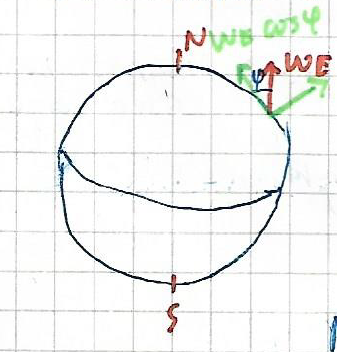
\includegraphics[width=0.65\textwidth]{EinflussBreite.png}}
\end{figure*}
\begin{gather*}
	\omega_E = Erddrehung \\
	\varepsilon = Kreiseldrehung \\
	M = I_w \cdot \omega_E \cdot \cos(\varphi)
\end{gather*}
2) Einfluss der Auslenkung (Kreiselazimuth)
\begin{figure*}[ht]\centering
	\subfigure[Einfluss der Auslenkung]{
		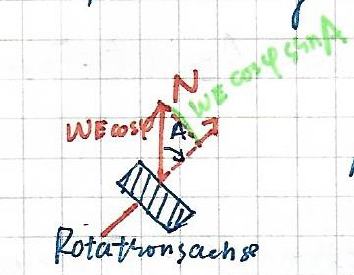
\includegraphics[width=0.65\textwidth]{EinflussAuslenkung.png}}
\end{figure*}
Gesamt Drehmoment:
\begin{equation*}
	D = I_w \cdot \omega_E \cdot \cos(\varphi) \cdot \sin(A)
\end{equation*}
Drehmoment / Präzessionsgeschwindigkeit wird umso größer:
\begin{itemize}
	\item je größer die Auslenkung $A$
	\item je größer die geographische Brete $\varphi$ \newline
	bei $\cos(\varphi) = 1$ um Äquator maximal \newline
	am Pol $\cos(\varphi) = 0$ Kein Drehmoment. \newline
	in der Praxis $|\varphi| \leq 75°$
\end{itemize}
Problem: Massenträgheit schwingt der Kreisel um den Meridianen.
\begin{itemize}
	\item Schwingungsdauer $T_0$ hängt von Konstruktionsprinzip ab
	\begin{equation*}
		T \approx \frac{T_0}{\sqrt{\cos(\varphi)}}
	\end{equation*}
	breitenabhängig.
\end{itemize}
\subsubsection{Bauformen und Gerätesysteme}
\subsubsection{Messverfahren}
Kreiselschwingung ist durch Ablesereinrichtung und Lichtzeigen ablesbar:
\begin{figure*}[ht]\centering
	\subfigure[]{
		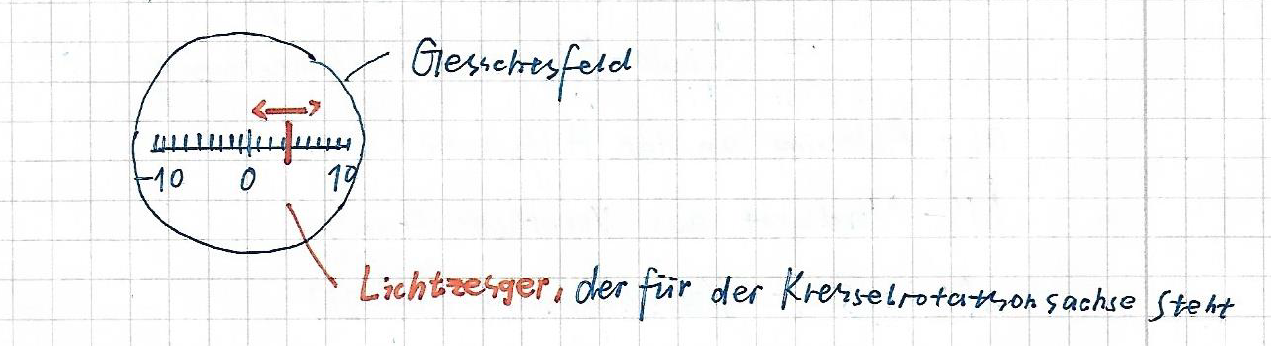
\includegraphics[width=0.65\textwidth]{Ableser.png}}
\end{figure*}
\newline
1) Schnellorientierung
\begin{itemize}
	\item Grobverfahren auf $0,05$ gon
	\item Nachführen des Lichtzeigens auf der Skalermittel durch Drehen der Alhidade(Theodolitoberbau) bis zu den Umkehrpunkte $v_W$ und $v_E$
	\item An der Umkehrpunkte die Ablesung $A_W$(West) und $A_E$(Ost) durchführen
	\item $N = \frac{A_E + A_W}{2}$
	\item Mittelwert $N$ aus Theodolit einstellen
	\item Nordwert $N$ ist ungenau, die die Schwingung gedämpft ist.
\end{itemize}
2) Umkehrpunktmethode
\begin{itemize}
	\item Feinorientierung $\sigma_N = 5 - 10$ mgon bei 4 bis 6 Umkehrpunkten
\end{itemize}
a) Mit nachführen:
\begin{itemize}
	\item Drehe der Alhidade führt zum Holten das Lichtzeiger in der Skalarmitte
	\item Ablesen des Teilkreisens an den Umkehrpunkten
	\item aus jeweils 3 Messungen das Schulen-Mittelbilden
\end{itemize}
Vorteile:
\begin{itemize}
	\item Vororientierung von geringer Bedeutung 
\end{itemize}
Nachteile:
\begin{itemize}
	\item Umkehrpunkten unsicher ablesbar
	\item Nachführen erforderlich
\end{itemize}
b) Ohne nachführen
\begin{itemize}
	\item Ablesung der Umkehrpunkten an den Hilfskalar
	\item Bildung des Schulemittels aus Hilfsskalarmitte, danach Transformation in Teilkreiswerte
	\item Diesmal schwingt der Lichtzeiger im Gesichtsfeld. Hierfür muss die Vorientierung sehr gut sein. bzw. der Kreisel machanisch abgebremst werden.
\end{itemize}
Parameter
\begin{itemize}
	\item $a_i$: Ablesung an der Hilfsskala in $s_E$
	\item $N'$: Nordwert aus Vororientierung
	\item $\Delta N = c \cdot S$: Korrkturwert aus 2b)
	\item $c$: Gerätekonstante/Umrechnunsfaktor 
\end{itemize}
Vorteile:
\begin{itemize}
	\item Kein Nachführung
	\item gut automatisiert
\end{itemize}
\begin{itemize}
	\item gute Vororienntierung erforderlich
	\item zum Teil mechanisches Abbremsen nötig
\end{itemize}
3) Durchgangsmethode
\begin{itemize}
	\item Feinorientierung
	\item $G_N = 5-10$ mgon bei $4-5$ Durchgängen
	\item Vororientierung und Abbremsen wie bei 2b)
	\item Beobachten von Durchgangszeiten $t_i$ des Lichtzeigers durch Skalennull mit der Stoppuhr
	\item Zusätzliche Ablesung der Amplituden an der Hilfsskala
	\begin{gather*}
		T_{E,i} = t_{2i} - t_{2i-1}\qquad T_{W,i} = t_{2i+1} - t_{2i} \\
		T_E = \frac{1}{m} \sum_{i=1}^{m} T_{E_i} \qquad T_W = \frac{1}{m} \sum_{i=1}^{m} T_{W_i} \\
		m =\frac{n}{2} - 1 \\
		T_E = \frac{T}{2} + 2 \delta T \qquad T_W = \frac{T}{2} - 2 \cdot \delta T \\
		\Longrightarrow T_E - T_W = 4 \cdot \delta T \\
		\Longrightarrow \delta T = \frac{T_E - T_W}{4} \\
		und:\; T = T_E + T_W \\
	\end{gather*}
	Amplituden aus Hilfsskala
	\begin{gather*}
		a = \frac{a_E - a_W}{2} \\
		S = a \cdot \sin(2\pi \cdot \frac{\delta T}{T}) \rightarrow S = a \cdot 2\pi \cdot \frac{\delta T}{T}\\
		N = N' + c \cdot S
	\end{gather*}
\end{itemize}
Vorteile:
\begin{itemize}
	\item Kein Nachführen erforderlich
	\item Durchgänge präziser beobachtbar
	\item automatisiertbar
\end{itemize}
Nachteile:
\begin{itemize}
	\item gute Vororientierung notwendig
	\item mechanisches Abbremsen schwierig
	\item Stoppuhr notwendig
\end{itemize}
4) Schwingungsintegration (für Kreiseltheodolite)
\begin{gather*}
	\Delta N = \frac{1}{T} \int_{t_0}^{t_1} \Delta N(t) dt \approx \frac{1}{n} \sum_{k=1}^{n} \Delta N_k
\end{gather*}
Vorteile
\begin{itemize}
	\item Kein Nachführen, keine Stoppuhr
	\item Komplett automatisiert
	\item höchste Genauigkeit: ca. 1mgon
\end{itemize}
\subsubsection{Korrektionen und Reduktion}
1) Korrektion
a) Gerätekonstante $E$
\begin{itemize}
	\item Abweichung der Nullmarken der Skala gegenüber dem Momentanpol (Nullpunktfehler)
	\item Bestimmung Kreiseln aus Soll-Azimuts
\end{itemize}
b) Fehlwinkel $\alpha$
\begin{itemize}
	\item nur bei Aufsatzkreiseln 
	\item zwischen Kreisellage und Zielfernrohr des Theodolites
\end{itemize}
c) In der Regel werden $E$ und $\alpha$ In einem Wert zusammengefasst
\begin{equation*}
A_m = \bar{z} - N + E - \alpha \Longrightarrow A_m = \bar{z} - N + E
\end{equation*}
2) Reduktion \newline
a) Polbewegung 
\begin{itemize}
	\item CIO: Conventional International Origin
	\item Astromisches Azimut: $A = A_m - \beta$
	\item Polreduktion: $\beta = \frac{x_p}{den}$
	\item aktuelle Polkoordiate: $x_P$, $y_P$
	\item astronomische Standpunktkoordinate: $\Lambda_S, \Phi_S$
	\item Querkrümmungsradius der Erde: $R$
\end{itemize}
Abschätzung: 
\begin{itemize}
	\item Polschwankung $<0,3''$
	\item $\Rightarrow \beta < 0,15$mgon
	\item vernachlässigbar
\end{itemize}
b) Übergang zum Ellipsoid
\begin{itemize}
	\item Ellipsoidisches Azimut $\alpha = A + \varepsilon$
	\item Laplace-Reduktion(verkürzt): $\varepsilon = -\eta \tan(\Phi_S)$
	\item Komponente der Lotabweichung: $\eta = (\Lambda - \lambda)\cos(\varphi)$,($\Phi_S$ kann durch $\phi_S$ ersetzt werden)
\end{itemize}
Abschätzung: (mit $z=100$gon, und $h_z \leq 1$km)
\begin{itemize}
	\item $\varepsilon \leq 1$mgon
\end{itemize}
Bei Gyromat zu berücksichtigen \newline
Bei Fennel TK4 nicht berücksichtigen \newline
\newline
c) Übergang in die Ebene
\begin{itemize}
	\item Richtungswinkel: $T = \alpha - \gamma$
	\item Meridiankonvergenz: $\gamma = (\lambda_s - \lambda_0) \cdot \sin(\varphi_s) = \frac{200gon}{\pi R} y_s \tan(\varphi_s)$
	\item ellipsoidische Breite des Standpunkts: $y_s$
	\item ellipsoidische Länge des Standpunkts, des Zentralmeridians: $\lambda_s$, $\lambda_0$
	\item Abstand des Standpunkts von Zentralmeridian im UTM-System
\end{itemize}
Abschätzung:
\begin{gather*}
	\varphi_s = 49° \\
	\lambda_s - \lambda_0 \leq 1,5° \\
	\Rightarrow \gamma = 1,25gon \\
	\Rightarrow wichtigste\; Reduktion
\end{gather*}
d) Berücksichtigung der Abbildungsreduktion
\begin{itemize}
	\item Richtungswinkel: $t = T - \delta$
	\item Richtungsreduktion $\delta = \frac{\rho}{b \cdot R^2} (x_z - x_s) \cdot (2y_s + y_z)$
	\item Zielpunkt: $x_z$, $y_z$
	\item Standpunkt: $x_s$, $y_s$
\end{itemize}
Abschätzung:
\begin{gather*}
	y_s = y_z < 100km \\
	x_z - x_s < 1km \\
	\Rightarrow \sigma < 0,08mgon \\
	\Rightarrow ohne\; Bedeutung \\
	\Rightarrow T = t
\end{gather*}
Zusammenfassung
\begin{itemize}
	\item Gyromat: $t = A + \varepsilon - \gamma$
	\item Fennel: $t = A - \gamma$
\end{itemize}
\subsection{Bestimmung des Durchschlagspunktes}
\end{document}
